\section{自适应步长}
\label{sec:odenum-adaptive}

固定步长要在全程迁就最难走的一段。解在某处急转，别处平缓，均匀的小步长就是浪费，均匀的大步长又不够准。程序能不能边走边判断，自己决定每一步走多远？

\paragraph{主要思想：估计局部误差}
要调节步长，先要知道这一步的误差有多大。真解未知，但可以用两个不同精度的结果相减来估计。

一种办法是\term{步长加倍}（step doubling）。设方法的阶为$p$，从同一点出发，用步长$h$走一步得到$\bm{y}_1$，用步长$h/2$走两步得到$\bm{y}_2$。忽略高阶项，两者的误差主要部分分别是$\bm{c}h^{p+1}$和$2\bm{c}(h/2)^{p+1}$，相减消去未知的真解，得到对$\bm{y}_2$的误差估计
\begin{equation}
 \bm{x}(t+h)-\bm{y}_2\approx\frac{\bm{y}_2-\bm{y}_1}{2^{p}-1}.
 \label{eq:odenum-step-doubling}
\end{equation}

例~\eqref{eq:odenum-running}的第一步，Euler方法用$h=0.5$得$0.28$，用两个$0.25$的半步得$0.2856$，由式~\eqref{eq:odenum-step-doubling}估计真解比$0.2856$约大$0.0056$。实际差是$0.291875-0.2856=0.0063$，估计相当准确。这种做法要多算一倍的步，代价偏高。

另一种办法用同一组阶段斜率组合出两个不同阶的结果，它们的差就是误差估计，不增加右端求值，这样的方法称为\term{嵌入式Runge--Kutta方法}（embedded Runge--Kutta method）。最简单的例子是Heun--Euler对。

取Heun方法的两个斜率$\bm{k}_1=\bm{f}(t,\bm{x})$，$\bm{k}_2=\bm{f}(t+h,\bm{x}+h\bm{k}_1)$。一阶的结果只用$\bm{k}_1$，二阶的结果用两者平均：
\[
 \bm{x}_{\mathrm{low}}=\bm{x}+h\bm{k}_1,\qquad
 \bm{x}_{\mathrm{high}}=\bm{x}+\frac{h}{2}(\bm{k}_1+\bm{k}_2).
\]
两者之差估计低阶结果的误差：
\begin{equation}
 \bm{d}=\bm{x}_{\mathrm{high}}-\bm{x}_{\mathrm{low}}=\frac{h}{2}(\bm{k}_2-\bm{k}_1).
 \label{eq:odenum-embedded-estimate}
\end{equation}
实际使用的是更高阶的配对，例如Dormand--Prince的五四阶方法\scite{math-hairer1993ode}，原理相同。

\paragraph{主要思想：尺度、接受与新步长}
误差估计要和一个容许的尺度比较。各分量量纲可能不同，大小也可能相差很多，所以给每个分量一个尺度，同时用\term{绝对容差}（absolute tolerance）$\eta_{\mathrm{a}}$和\term{相对容差}（relative tolerance）$\eta_{\mathrm{r}}$：
\begin{equation}
 w_i=\eta_{\mathrm{a}}+\eta_{\mathrm{r}}\max\bigl\{\lvert x_i\rvert,\ \lvert x_{\mathrm{high},i}\rvert\bigr\}.
 \label{eq:odenum-scale}
\end{equation}
相对容差让大分量按比例控制精度；绝对容差防止分量接近零时尺度也趋于零，把步长压到不合理的小。

归一化的误差取各分量比值的最大值：
\begin{equation}
 \mathrm{err}=\max_{i}\frac{\lvert d_i\rvert}{w_i}.
 \label{eq:odenum-err}
\end{equation}
若$\mathrm{err}\leq1$，这一步被接受，否则放弃这一步，用更小的步长重算。

无论接受与否，都要决定下一个步长。低阶结果的阶为$q$时，$\mathrm{err}$大约正比于$h^{q+1}$，要让它变成$1$，步长应乘以$\mathrm{err}^{-1/(q+1)}$。加上安全系数$\gamma<1$和增减幅度的限制，得到
\begin{equation}
 h_{\mathrm{new}}=h\,\min\Bigl\{f_{\max},\ \max\bigl\{f_{\min},\ \gamma\,\mathrm{err}^{-1/(q+1)}\bigr\}\Bigr\}.
 \label{eq:odenum-step-control}
\end{equation}
限制幅度是因为$\mathrm{err}$只是估计，步长剧烈变化会使估计失效。

\paragraph{计算过程}
下面用例~\eqref{eq:odenum-running}演示Heun--Euler对，$q=1$，取容差和控制参数为
\[
 \eta_{\mathrm{a}}=\eta_{\mathrm{r}}=10^{-3},\quad\gamma=0.9,\quad f_{\min}=0.2,\quad f_{\max}=5,
\]
初始步长取$h=0.5$，积分到$T=1$，接受后沿用高阶结果继续。

\needspace{6\baselineskip}
\paragraph{变量}
\begin{itemize}
 \item $t$，$\bm{x}\in\mathbb{R}^{n}$：已接受的当前时刻和数值解。
 \item $h$：当前尝试的步长。
 \item $\bm{k}_1,\bm{k}_2\in\mathbb{R}^{n}$：本次尝试的两个阶段斜率。
 \item $\bm{d}$，$\mathrm{err}$：误差估计和归一化误差。
 \item 标记$\mathrm{failed}$：上一次尝试是否被拒绝，被拒绝后下一步的$f_{\max}$取$1$，避免紧接着又放大步长。
\end{itemize}

\paragraph{初始化}
把当前点初始化为初值，并设初始步长。例中
\[
 t=0,\qquad x=0.2,\qquad h=0.5,\qquad \mathrm{failed}=\text{否}.
\]

\needspace{6\baselineskip}
\paragraph{每轮更新}
当$t<T$时重复：
\begin{enumerate}

 \item \textbf{截断到终点。}令$h\leftarrow\min\{h,T-t\}$，保证不越过$T$。

 \item \textbf{算两个斜率和两个结果。}计算$\bm{k}_1,\bm{k}_2$，$\bm{x}_{\mathrm{high}}$，并由式~\eqref{eq:odenum-embedded-estimate}算$\bm{d}$。例中第一次尝试
 \[
  k_1=0.16,\qquad k_2=f(0.28)=0.2016,
 \]
 于是
 \[
  x_{\mathrm{high}}=0.2904,\qquad d=0.25\times0.0416=0.0104.
 \]

 \item \textbf{比较尺度。}由式~\eqref{eq:odenum-scale}和式~\eqref{eq:odenum-err}计算$\mathrm{err}$。例中第一次尝试
 \[
  w=10^{-3}+10^{-3}\times0.2904=0.00129,\qquad \mathrm{err}=8.06.
 \]

 \item \textbf{接受或拒绝。}若$\mathrm{err}\leq1$，令$t\leftarrow t+h$，$\bm{x}\leftarrow\bm{x}_{\mathrm{high}}$，$\mathrm{failed}$置为否；否则状态不变，$\mathrm{failed}$置为是。例中第一次$\mathrm{err}>1$，拒绝，状态仍为$(0,\,0.2)$。

 \item \textbf{更新步长。}由式~\eqref{eq:odenum-step-control}计算$h_{\mathrm{new}}$，令$h\leftarrow h_{\mathrm{new}}$。例中第一次尝试
 \[
  h_{\mathrm{new}}=0.5\times\max\bigl\{0.2,\ 0.9\times8.06^{-1/2}\bigr\}=0.5\times0.317=0.1585.
 \]
 例中第二次尝试用$h=0.1585$，得到
 \[
  k_2=0.174574,\qquad x_{\mathrm{high}}=0.226517,\qquad \mathrm{err}=0.942,
 \]
 这一步被接受，$t$更新为$0.1585$，$x$更新为$0.226517$。

 \item \textbf{停止。}当$t=T$时结束。
\end{enumerate}
全程的尝试列于表~\ref{tab:odenum-adaptive-trace}。一共$8$次尝试、$16$次右端求值，一次被拒绝；最终$x=0.404269$，真值$0.404610$，全局误差$-3.4\times10^{-4}$。

\begin{BookInlineTable}
 \centering
 \caption{Heun--Euler对在式~\eqref{eq:odenum-running}上的步长控制，$\eta_{\mathrm{a}}=\eta_{\mathrm{r}}=10^{-3}$。最后一步被截断以恰好到达$T=1$。}
 \label{tab:odenum-adaptive-trace}
 \begin{tabular}{rrrrc}
  \toprule
  $t$ & $h$ & $x_{\mathrm{high}}$ & $\mathrm{err}$ & 结果\\
  \midrule
  0 & 0.50000 & 0.290400 & 8.060 & 拒绝\\
  0 & 0.15851 & 0.226517 & 0.942 & 接受\\
  0.15851 & 0.14701 & 0.253260 & 0.787 & 接受\\
  0.30552 & 0.14911 & 0.282437 & 0.763 & 接受\\
  0.45462 & 0.15366 & 0.314545 & 0.735 & 接受\\
  0.60828 & 0.16128 & 0.350259 & 0.698 & 接受\\
  0.76956 & 0.17373 & 0.390689 & 0.642 & 接受\\
  0.94329 & 0.05671 & 0.404269 & 0.056 & 接受\\
  \bottomrule
 \end{tabular}
\end{BookInlineTable}

\paragraph{步长怎样跟随解}
图~\ref{fig:odenum-adaptive-steps}是同一控制器用在变化更剧烈的方程$\dot{x}=12x(1-x)$上的结果，$x(0)=0.02$，容差仍为$10^{-3}$。解从缓慢上升到快速爬升，再到贴近平衡点。控制器在曲线转弯的区域用小步，在平衡点附近把步长放大，共接受$49$步、拒绝$6$步，$110$次右端求值，终点误差约$5\times10^{-4}$。

\begin{BookInlineFigure}
 \centering
 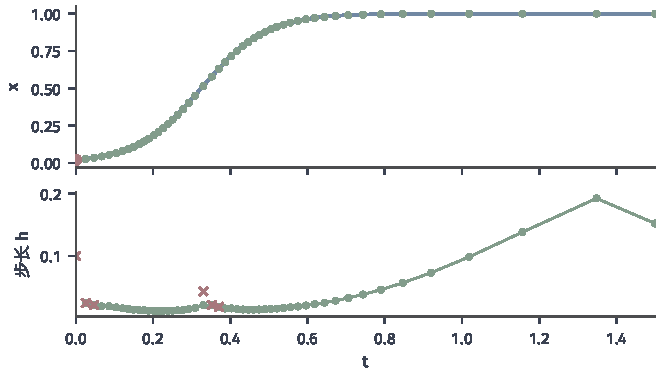
\includegraphics[width=112mm]{figures/06-differential-equations/01-ordinary-differential-equations/matplotlib/odenum-adaptive-steps/figure.pdf}
 \caption{自适应步长跟随解的变化，方程$\dot{x}=12x(1-x)$，$x(0)=0.02$，$\eta_{\mathrm{a}}=\eta_{\mathrm{r}}=10^{-3}$。上图蓝线是真解，红点是初值，绿点是接受的网格值；下图绿线是接受步的步长，红叉是被拒绝的尝试。}
 \label{fig:odenum-adaptive-steps}
\end{BookInlineFigure}

\paragraph{局部容差不直接保证全局精度}
控制器管的是每一步新增的偏差，全局误差还要乘上流映射的放大。回到第~\ref{sec:odenum-time-discretization}节的方程$\dot{x}=\sigma(x-\cos t)-\sin t$，$x(0)=1$，积分到$T=2$。图~\ref{fig:odenum-adaptive-global}显示，同样的局部容差，$\sigma=-5$时全局误差大致等于容差，$\sigma=5$时放大了四个多数量级。容差取$10^{-5}$时，前者的全局误差约$6\times10^{-6}$，后者约$0.18$。

\begin{BookInlineFigure}
 \centering
 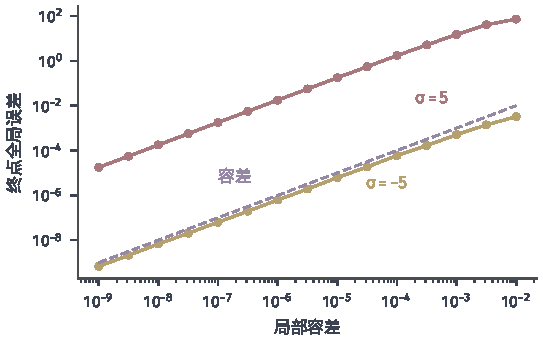
\includegraphics[width=92mm]{figures/06-differential-equations/01-ordinary-differential-equations/matplotlib/odenum-adaptive-global/figure.pdf}
 \caption{局部容差与终点全局误差，方程为$\dot{x}=\sigma(x-\cos t)-\sin t$，$x(0)=1$，$T=2$，$\eta_{\mathrm{a}}=\eta_{\mathrm{r}}$。黄线$\sigma=-5$，红线$\sigma=5$，紫色虚线为容差本身。}
 \label{fig:odenum-adaptive-global}
\end{BookInlineFigure}

所以容差不是全局精度的保证。可靠的做法是把容差减小一两个数量级再解一次，比较两次的结果；或者用第~\ref{chap:ode-sensitivity}章的敏感性信息估计放大因子。这样的比较检验的是数值误差，并不能发现模型本身的错误。

\paragraph{自适应不能解决刚性}
控制器还会被稳定性牵着走。把Heun--Euler对用于系统~\eqref{eq:odenum-stiff-system}，容差$10^{-3}$，走到$T=4$。快速过渡结束后，解已经很平缓，局部误差估计却不断地“被激发”：一旦步长越过稳定上限，快速模式开始放大，误差估计变大，步长又被压回来。

结果是步长一直贴着上限$2/50$上下摆动（图~\ref{fig:odenum-adaptive-stiff}）。共接受$141$步、拒绝$13$步，$308$次右端求值，后半程的平均步长约$0.039$，而精度本来允许走得更远。

\begin{BookInlineFigure}
 \centering
 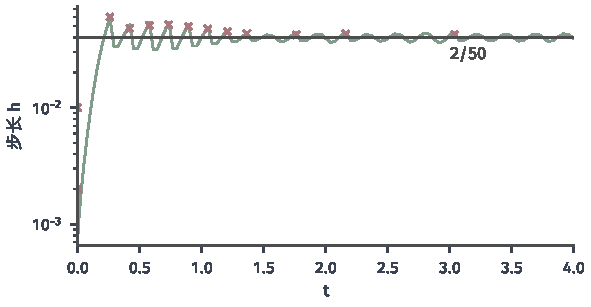
\includegraphics[width=100mm]{figures/06-differential-equations/01-ordinary-differential-equations/matplotlib/odenum-adaptive-stiff/figure.pdf}
 \caption{显式嵌入对用于刚性系统~\eqref{eq:odenum-stiff-system}时的步长历史，容差$10^{-3}$。绿线是接受步的步长，红叉是被拒绝的尝试，深灰线是稳定上限$2/50$。解变平缓之后，步长仍被稳定性限制。}
 \label{fig:odenum-adaptive-stiff}
\end{BookInlineFigure}

步长长期贴着一个与解的光滑程度无关的水平，同时反复被拒绝，这本身就是刚性的信号，应当换成隐式方法。求值次数的增长同样值得监控：它比预期多很多时，要么是方程刚性，要么是右端有不连续点，控制器把步长压小只是在逼近那一点，并不能恢复方法的阶。

